

%(BEGIN_QUESTION)
% Copyright 2007, Tony R. Kuphaldt, released under the Creative Commons Attribution License (v 1.0)
% This means you may do almost anything with this work of mine, so long as you give me proper credit

Se på denne P\&ID-en:

$$\includegraphics[width=15.5cm]{rk001x01.eps}$$

Begge pumpene er stempelpumper, en form for fortrengingspumpe. Den vil pumpe et bestemt volum for hver rotasjon. 

Hva vil skje med nivået i beholderen om en av pumpene  pumper mer en den andre?
 
\vskip 10pt

Vil du kalle dette for en integrerende eller selvstabiliserende prosess?

\underbar{file rk001.tex}
%\underbar{file i01658}
%(END_QUESTION)





%(BEGIN_ANSWER)

The liquid level inside the vessel will drift either up or down (depending on which pump moves more liquid) at a rate determined by the differential liquid flow ($Q_{in}$ $-$ $Q_{out}$).  This makes it an {\it integrating} process.

\vskip 10pt

Integrating processes are characterized by the capacity to experience persistent mass and/or energy imbalances, where the out-flow of mass and/or energy does not naturally reach equilibrium the in-flow over time.  Self-regulating processes, by contrast, naturally equalize their mass and energy balances as the process variable changes.

%(END_ANSWER)





%(BEGIN_NOTES)


%INDEX% Control, process characteristics: self-regulating versus integrating

%(END_NOTES)


